\documentclass{beamer}
	
	\usepackage[utf8]{inputenc} 
	\usepackage[T1]{fontenc}      
	\usepackage[francais]{babel}
	\usepackage[absolute,overlay]{textpos}
	\usepackage{graphicx}
	
	\graphicspath{figures/}
	
	\useoutertheme{shadow}% Pied de page
	\usetheme{PaloAlto}% Thème avec sidebar
	
	%\setbeamercolor{structure}{fg=cyan}
	
	% Mise en forme pour la première diapo
	\title[Présentation]{Retrogaming : Metal Slug}
	\subtitle[\ldots]{Soutenance Projet}
	\author[BONNIN GIRARD SILOTIA WAGNER]{Thomas BONNIN Jules GIRARD \\ Gilles SILOTIA Pascal WAGNER}
	\institute[UM2]{Université de Montpellier}
	\institute[UM2]{Université de Montpellier \\ Faculté des Sciences}
	\date{\today}
	
	% Retire les noms et titre de la sidebar
	\makeatletter
		\setbeamertemplate{sidebar \beamer@sidebarside}%{sidebar theme}
		{
			\beamer@tempdim=\beamer@sidebarwidth%
			\advance\beamer@tempdim by -6pt%
			\insertverticalnavigation{\beamer@sidebarwidth}%
			\vfill
			\ifx\beamer@sidebarside\beamer@lefttext%
			\else%
				\usebeamercolor{normal text}%
				\llap{\usebeamertemplate***{navigation symbols}\hskip0.1cm}%
				\vskip2pt%
			\fi%
		}%
	\makeatother
	
	% Numéro de diapo (en com rajoute le nombre de diapos au total -> 1/20 ... 20/20)
	\addtobeamertemplate{footline}{\insertframenumber}%/\inserttotalframenumber}
	
	% Insère une diapo à chaque changement de section comportant le sommaire
	% avec la nouvelle section courante (et ses sous-sections) en noir et
	% le reste en grisé/transparent
	\AtBeginSection[]
	{
		\begin{frame}
			\frametitle{Sommaire}
			\tableofcontents[currentsection, hideothersubsections]
		\end{frame} 
	}

	\begin{document}
		
		% Première diapo sans sidebar [plain] et centrer
		\begingroup
			\makeatletter
				\setlength{\hoffset}{-.5\beamer@sidebarwidth}
			\makeatother
			\begin{frame}[plain]
				\begin{textblock*}{2cm}(2cm,6cm) % {block width} (coords)
					
\includegraphics[width=2cm]{figures/logo_fds.png}
				\end{textblock*}
				\begin{textblock*}{2.25cm}(10cm,6cm) % {block width} (coords)
					
\includegraphics[width=2.25cm]{figures/logo_um.png}
				\end{textblock*}
				\titlepage
			\end{frame}
		\endgroup
		
		% Deuxième diapo annonce du plan
		\begin{frame}
			% Titre diapo
			\frametitle{Sommaire}
			% Plan sans sous-sections
			\tableofcontents[hideallsubsections]
		\end{frame}
		
		
		%%%%%%%%%%%%%%%%%%%%%%%%%%%%%%%%%%%%%%%%%%%%%%%%%%%%%%%%%%%%%%
		%%%														   %%%
		%%%	Les diapos qui suivent (avant la première section) ne  %%%
		%%%	sont que des tests et des exemples pour nous aider     %%%
		%%%														   %%%
		%%%%%%%%%%%%%%%%%%%%%%%%%%%%%%%%%%%%%%%%%%%%%%%%%%%%%%%%%%%%%%
		
		
		% Quelques mises en forme avec des beaux cadres
		\begin{frame}
			\begin{block}{Qu'est-ce un bloc sous Beamer ?}
				Tout simplement ceci !
			\end{block}
			\begin{definition} % Définition
				On donne une définition.
			\end{definition}

			\begin{example} % Exemple
				Suivi d'un exemple.
			\end{example}

			\begin{theorem} % Théorème
				On peut éventuellement ajouter un théorème.
			\end{theorem}

			\begin{proof} % Démonstration
				Suivi de sa démonstration.
			\end{proof}
		\end{frame}
		
		
		\begin{frame}
			\frametitle{Un exemple de titre}
			\framesubtitle{avec un exemple de sous-titre}
			Enfin, le texte ! :)
		\end{frame}
		
		% Considérer comme une même diapo mais avec des animations
		\begin{frame}
			\begin{itemize}
				\item<1,3> Ploum!
				\item<2-4> Plim?
				\item Plum...
			\end{itemize}
		\end{frame}
		
		
		
		
		
		
		% Introduction
		\section{Introduction}
		\begin{frame}
	%%%%%%%%%%%%%%%%%%%% ECHELLE %%%%%%%%%%%%%%%%%%%%
	
	%% origine %%
	\begin{textblock*}{0cm}(0cm,0cm)
		0
	\end{textblock*}
	
	%% x %%
	\begin{textblock*}{0cm}(1cm,0cm)
		1
	\end{textblock*}
	\begin{textblock*}{0cm}(2cm,0cm)
		2
	\end{textblock*}
	\begin{textblock*}{0cm}(3cm,0cm)
		3
	\end{textblock*}
	\begin{textblock*}{0cm}(4cm,0cm)
		4
	\end{textblock*}
	\begin{textblock*}{0cm}(5cm,0cm)
		5
	\end{textblock*}
	\begin{textblock*}{0cm}(6cm,0cm)
		6
	\end{textblock*}
	\begin{textblock*}{0cm}(7cm,0cm)
		7
	\end{textblock*}
	\begin{textblock*}{0cm}(8cm,0cm)
		8
	\end{textblock*}
	\begin{textblock*}{0cm}(9cm,0cm)
		9
	\end{textblock*}
	\begin{textblock*}{0cm}(10cm,0cm)
		10
	\end{textblock*}
	\begin{textblock*}{0cm}(11cm,0cm)
		11
	\end{textblock*}
	\begin{textblock*}{0cm}(12cm,0cm)
		12
	\end{textblock*}
	
	 %% y %%
	\begin{textblock*}{0cm}(0cm,1cm)
		1
	\end{textblock*}
	\begin{textblock*}{0cm}(0cm,2cm)
		2
	\end{textblock*}
	\begin{textblock*}{0cm}(0cm,3cm)
		3
	\end{textblock*}
	\begin{textblock*}{0cm}(0cm,4cm)
		4
	\end{textblock*}
	\begin{textblock*}{0cm}(0cm,5cm)
		5
	\end{textblock*}
	\begin{textblock*}{0cm}(0cm,6cm)
		6
	\end{textblock*}
	\begin{textblock*}{0cm}(0cm,7cm)
		7
	\end{textblock*}
	\begin{textblock*}{0cm}(0cm,8cm)
		8
	\end{textblock*}
	\begin{textblock*}{0cm}(0cm,9cm)
		9
	\end{textblock*}
	
	%%%%%%%%%%%%%%%%%%%%%%%%%%%%%%%%%%%%%%%%%%%%%%%%%
	
	\frametitle{Présentation générale du projet}
	
	
	
	\begin{textblock*}{5cm}(8cm,3cm)
		Conception d'un jeu rétro
	\end{textblock*}
	
	\begin{textblock*}{5cm}(2cm,5.25cm)
		Avec des outils modernes
	\end{textblock*}
	
	\only<2->
	{
		\begin{textblock*}{3cm}(2.5cm,2.5cm)
			
\includegraphics[width=3cm]{figures/logo_metal_slug.png}
		\end{textblock*}
	
		\begin{textblock*}{5cm}(8cm,3.5cm)
			\begin{itemize}
				\setbeamertemplate{itemize item}[triangle]
				\item Metal Slug
			\end{itemize}
		\end{textblock*}
	}
	
	\only<3->
	{
		\begin{textblock*}{5cm}(2cm,5.75cm)
			\begin{itemize}
				\item SFML
			\end{itemize}
			\begin{itemize}
				\item C++
			\end{itemize}
			\begin{itemize}
				\item MVC
			\end{itemize}
		\end{textblock*}
	
		\begin{textblock*}{3cm}(8cm,5.25cm)
			
\includegraphics[width=3cm]{figures/logo_sfml.png}
		\end{textblock*}
	
		\begin{textblock*}{3cm}(8cm,6.75cm)
			
\includegraphics[width=3cm]{figures/logo_c++.png}
		\end{textblock*}
	}
	
\end{frame}


\begin{frame}

	\frametitle{La licence Metal Slug}
	
	\begin{textblock*}{3cm}(5.75cm,4.25cm)
		
\includegraphics[width=3cm]{figures/logo_metal_slug.png}
	\end{textblock*}
	
	\only<2->
	{
		\begin{textblock*}{5cm}(6cm,2.5cm)
			Nazca / SNK
		\end{textblock*}
		\begin{textblock*}{5cm}(3.25cm,3.5cm)
			Shoot'em up
		\end{textblock*}
		\begin{textblock*}{5cm}(8.75cm,3.5cm)
			1996
		\end{textblock*}
		\begin{textblock*}{5cm}(1.75cm,5cm)
			Graphismes détaillés
		\end{textblock*}
		\begin{textblock*}{5cm}(9.25cm,5cm)
			Animations soignées
		\end{textblock*}
		\begin{textblock*}{5cm}(3.5cm,6.5cm)
			Easter eggs
		\end{textblock*}
		\begin{textblock*}{5cm}(8.75cm,6.5cm)
			Humour parodique
		\end{textblock*}
		\begin{textblock*}{5cm}(5.75cm,7.5cm)
			Action frénétique
		\end{textblock*}
	}
	
\end{frame}


\begin{frame}
	
\end{frame}


\begin{frame}
	
\end{frame}


		
		% Cahier des charges
		\section{Cahier des charges}
		\begin{frame}
	
\end{frame}


\begin{frame}
	
\end{frame}


\begin{frame}
	\frametitle{Spécifications fonctionnelles}
	\framesubtitle{Gameplay}
	\only<2>
	{
		\begin{textblock*}{8cm}(3.2cm,2.75cm)
			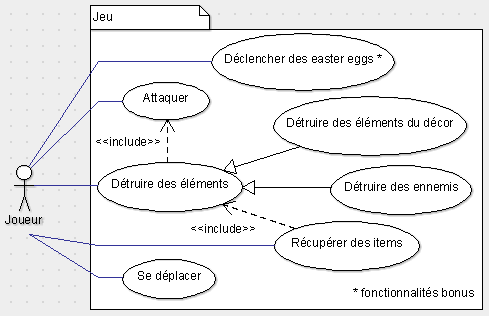
\includegraphics[width=8cm]{figures/use_case_metal_slug_gameplay.png}
		\end{textblock*}
	}
	\only<3>
	{
		\begin{textblock*}{9cm}(2.65cm,3.5cm)
			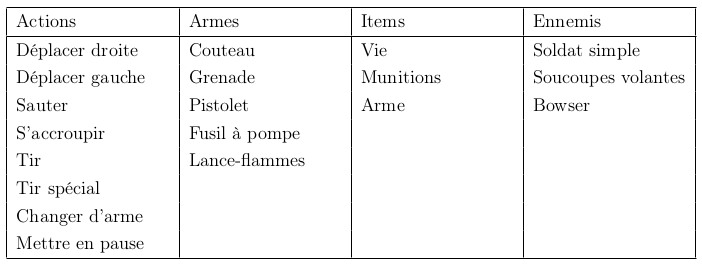
\includegraphics[width=9cm]{figures/tableau_gameplay.png}
		\end{textblock*}
	}
\end{frame}


\begin{frame}
	
\end{frame}


\begin{frame}
	
\end{frame}


		
		% Analyse
		\section{Analyse}
		\begin{frame}

	\frametitle{Analyse technique}
	\framesubtitle{Analyse de l'image}

	\begin{textblock*}{4.5cm}(2.5cm,2cm)
		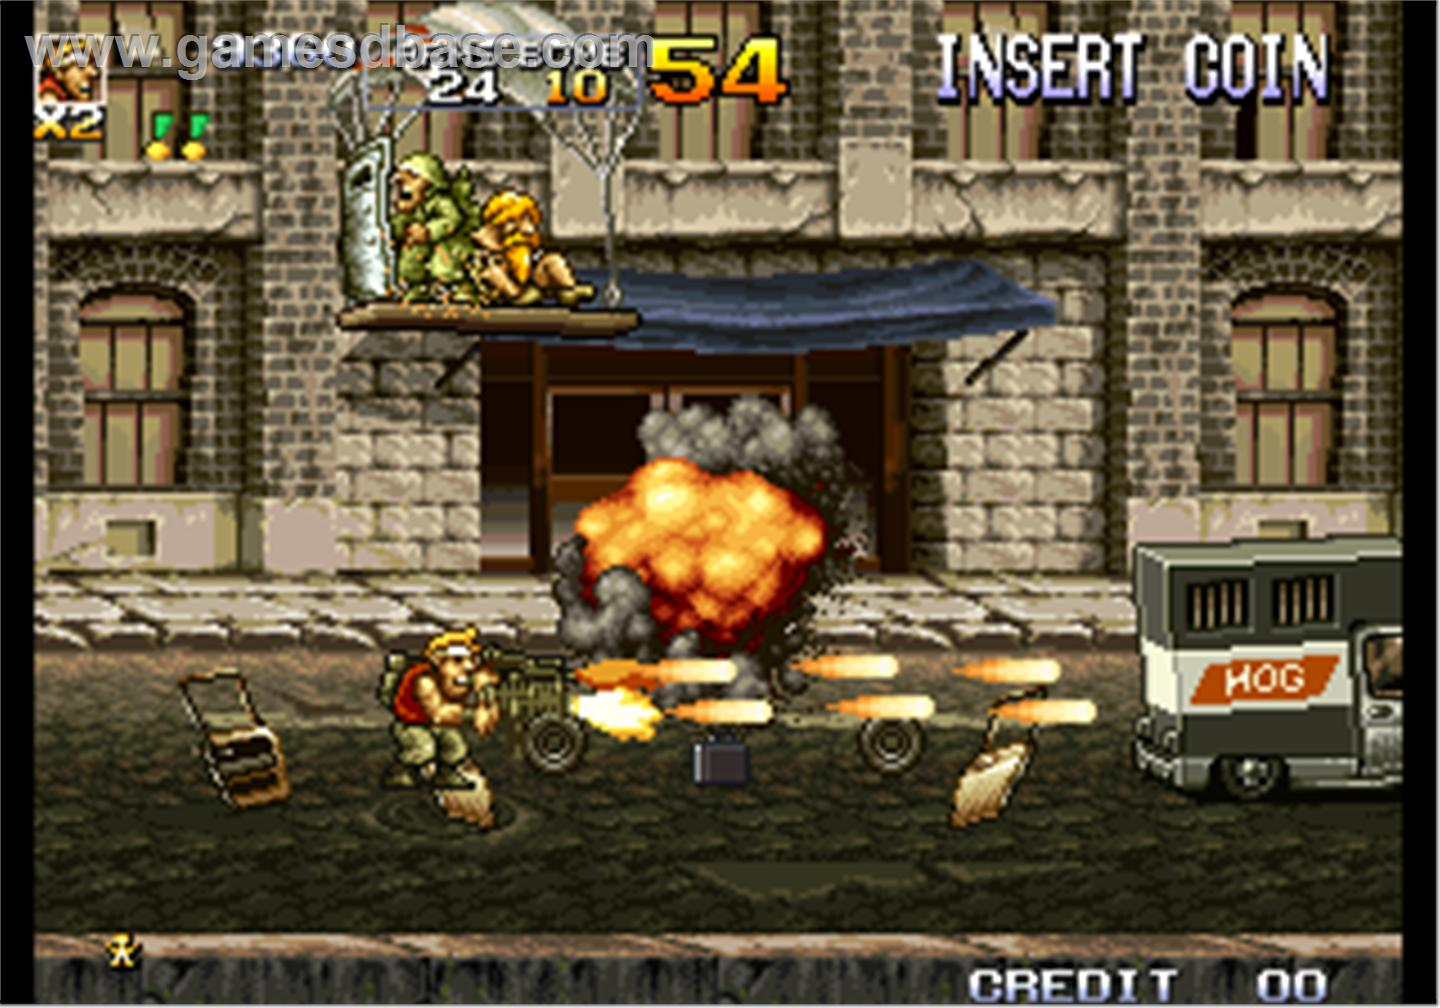
\includegraphics[width=4.5cm,height=3cm]{figures/screen_jeuorigine_1.jpg}
	\end{textblock*}

	\begin{textblock*}{4.5cm}(7.5cm,2cm)
		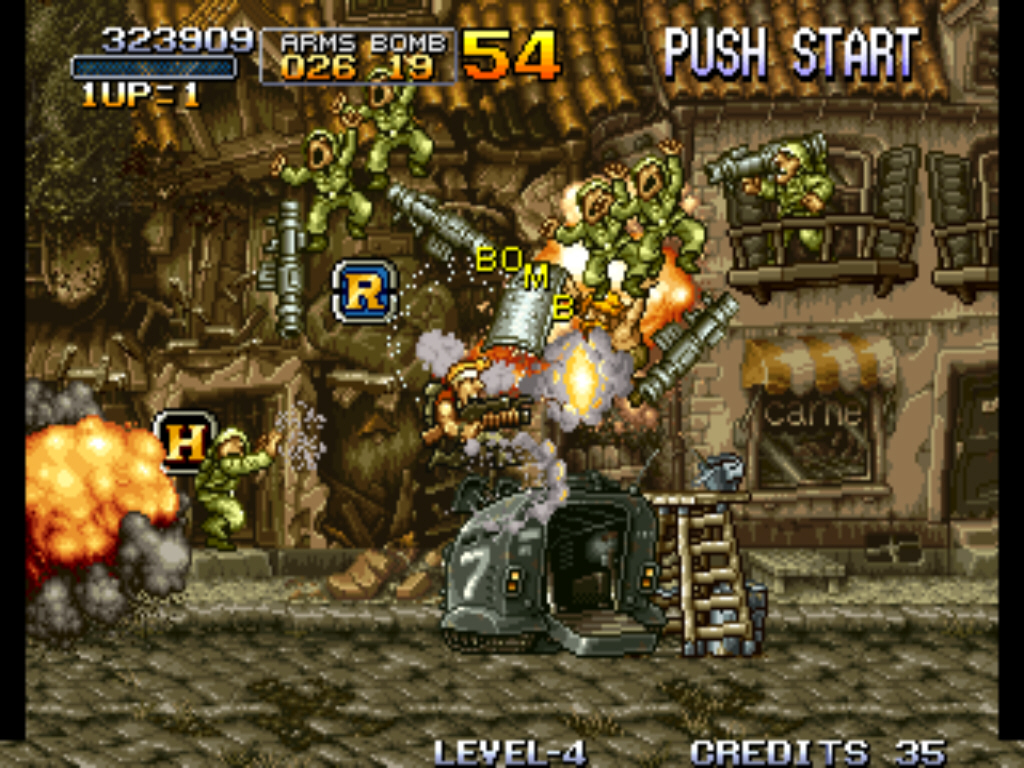
\includegraphics[width=4.5cm,height=3cm]{figures/screen_jeuorigine_2.jpg}
	\end{textblock*}

	\begin{textblock*}{4.5cm}(2.5cm,5.5cm)
		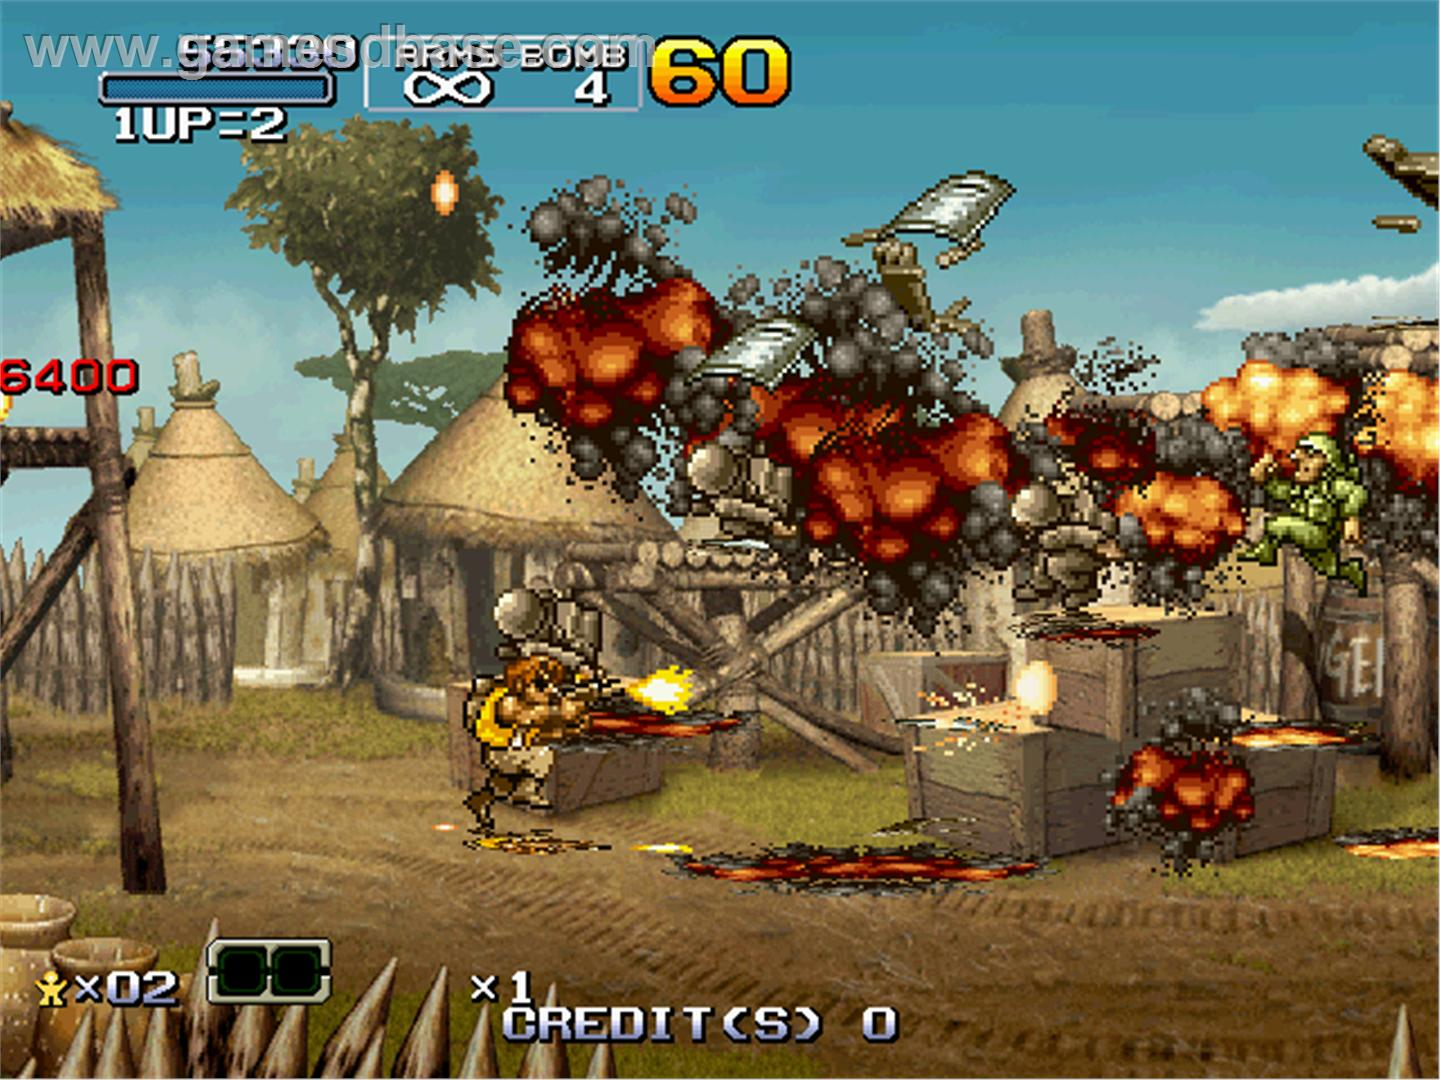
\includegraphics[width=4.5cm,height=3cm]{figures/screen_jeuorigine_3.jpg}
	\end{textblock*}

	\begin{textblock*}{4.5cm}(7.5cm,5.5cm)
		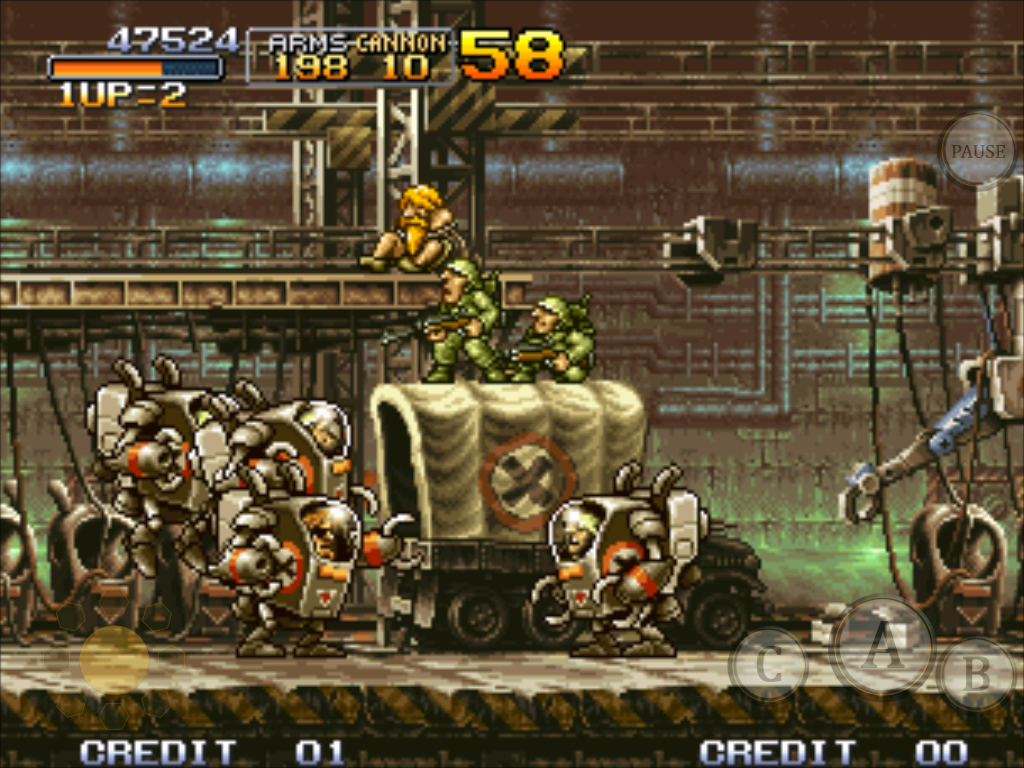
\includegraphics[width=4.5cm,height=3cm]{figures/screen_jeuorigine_4.png}
	\end{textblock*}

\end{frame}


\begin{frame}
	
\end{frame}


\begin{frame}

	\frametitle{Analyse technique}
	\framesubtitle{Gestion des collisions}

	\begin{textblock*}{3cm}(3.5cm,4cm)
		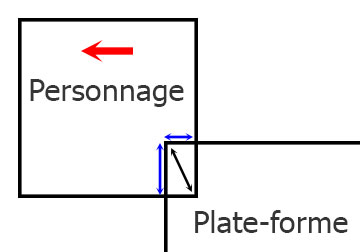
\includegraphics[width=3cm]{figures/collision_decalGauche.jpg}
	\end{textblock*}

	\begin{textblock*}{3cm}(7.5cm,4cm)
		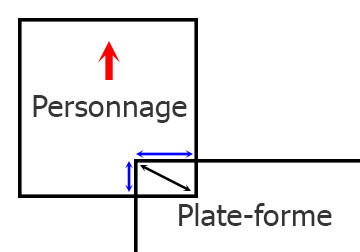
\includegraphics[width=3cm]{figures/collision_decalHaut.jpg}
	\end{textblock*}

\end{frame}


\begin{frame}

	\frametitle{Analyse et Conception}
	\framesubtitle{Animation}

	\begin{textblock*}{3cm}(3cm,2cm)
		
\includegraphics[width=8cm]{figures/partie_feuille_sprite.jpg}
	\end{textblock*}

	\begin{textblock*}{3cm}(4cm,7cm)
		
\includegraphics[width=6cm]{figures/xml_anim.png}
	\end{textblock*}

\end{frame}

\begin{frame}
	
\end{frame}


		
		% Conception/réalisations
		\section{Conception et réalisations}
		\begin{frame}

\frametitle{Améliorations et perspectives}
	\framesubtitle{Fonctionnalités manquantes}


	\begin{textblock*}{2.5cm}(9.5cm,4cm)
		
\includegraphics[width=2.5cm]{figures/vehicle.png}
	\end{textblock*}


	\begin{itemize}
		\item{Plus de types d'ennemis}
	\end{itemize}

	\begin{itemize}
		\item{Véhicules pilotables}
	\end{itemize}

	\begin{itemize}
		\item{Cinématiques}
	\end{itemize}

	
\end{frame}


\begin{frame}

\frametitle{Améliorations et perspectives}
	\framesubtitle{Améliorations possibles}


	\begin{textblock*}{2.5cm}(9cm,4cm)
		
\includegraphics[width=2.5cm]{figures/pad_xbox.png}
	\end{textblock*}


	\begin{itemize}
		\item Effets spéciaux supplémentaires
	\end{itemize}
	
	\begin{itemize}
		\item Support d'une manette de jeu
	\end{itemize}

	\begin{itemize}
		\item Ajout d'un mode multijoueur
	\end{itemize}
	

\end{frame}


\begin{frame}
	
\end{frame}


\begin{frame}
	
\end{frame}


\begin{frame}
	
\end{frame}


		 
		% Améliorations/Perspectives
		\section{Améliorations et perspectives}
		\begin{frame}

\frametitle{Conclusion}

	
	
	\begin{itemize}
		\item{Problèmes dans la gestion du projet}
	\end{itemize}

	\begin{itemize}
		\item{Quelques points de l'architecture à corriger}
	\end{itemize}

	\begin{itemize}
		\item{Jeu maintenable et évolutif}
	\end{itemize}
	


\end{frame}


\begin{frame}
	
\end{frame}


		
		% Conclusion
		\section{Conclusion}
		\begin{frame}
	
\end{frame}


\begin{frame}
	
\end{frame}


		
		
		
	\end{document}
